% !TEX root=../root.tex

To demonstrate the effectiveness of the proposed estimation algorithm, we first
present results from simulation.
% We present simulation results to demonstrate the effectiveness of the proposed estimation
% algorithm.
A multirotor UAV and a landing target vehicle were simulated using the dynamics presented
in~\eqref{eq:uav_dynamics} and~\eqref{eq:goal_dynamics} with the zero-mean
Gaussian noise processes as described
% The standard deviations used for the zero-mean
% Guassian noise processes in the dynamics are found
in~\tabref{tab:sim_process_noises}.
% As the estimator depends on
% tracking and estimating the positions of visual features that are rigidly
% attached to the landing vehicle, feature positions on the landing vehicle
Positions of visual features on the target vehicle
were also simulated by randomly sampling from the uniform distribution
% Positions for each feature in the goal frame are
% randomly sampled from the
% uniform distribution
\begin{equation}
  \vect{r}_{i/g}^g = \mathcal{U}
  \left( \begin{bmatrix} -2 \\ -2 \\ -1 \end{bmatrix},
  \begin{bmatrix} 2 \\ 2 \\ 1 \end{bmatrix} \right).
  \label{eq:uniform_dist}
\end{equation}
To emulate a visual feature tracker losing track of features, simulated features
randomly disappeared at each time step of the simulation.
% were randomly eliminated from the estimated state with a one percent probabilty 
% persisted to the next time step with a 99\% probability
When a feature disappeared, a new feature was generated by sampling
from~\eqref{eq:uniform_dist}
such that several
hundred, different features were used during a 30 second simulation.
% When a
% simulated feature was no longer tracked, a new feature was randomly generated by
% sampling from~\eqref{eq:uniform_dist}.
% one percent chance of 
% At each time step of the simulation, features are given a one percent chance
% of disappearing. When a feature disappears, a new feature is randomly
% generated by sampling from~\eqref{eq:uniform_dist}.

\begin{table}[htb!]
  \begin{center}
    \caption{Simulated Motion Model Parameters.}
    \label{tab:sim_process_noises}
    \begin{tabular}{l|l}
      \textbf{Parameter} & \textbf{Std. Deviation} \\
      \hline
      $\vect{\eta}_{\beta_a}$ & 0.05 m/s$^2$ \\
      $\vect{\eta}_{\beta_\omega}$ & 0.01 rad/s \\
      $\vect{\eta}_{gv}$ & 5 m/s \\
      $\vect{\eta}_{g\omega}$ & 5 rad/s \\
      % v & 5 m/s \\
      % landmark $x_{\text{min}}$ & -2 m \\
      % landmark $x_{\text{max}}$ & 2 m \\
      % landmark $y_{\text{min}}$ & -2 m \\
      % landmark $y_{\text{max}}$ & 2 m \\
      % landmark $z_{\text{min}}$ & -1 m \\
      % landmark $z_{\text{max}}$ & 1 m \\
      % landmark disappear prob. & 1\% \\
    \end{tabular}
  \end{center}
\end{table}

The initial state of the landing target vehicle was given by
\begin{equation}
  \begin{bmatrix}
    \vect{p}_{g/b}^v \\
    \vect{v}_{g/I}^g \\
    \psi_I^g \\
    \omega_{g/I}^g
  \end{bmatrix}
  =
  \begin{bmatrix}
    \begin{bmatrix} 0 & 0 & 5 \end{bmatrix}^\transpose \text{m} \\[1mm]
    % 0.5 \hphantom{\cdot} m/s \\
    \begin{bmatrix} 0.5 & 0.0 \end{bmatrix}^\transpose \text{m/s} \\
    1.5 \hphantom{\cdot} \text{rad} \\
    0.5 \hphantom{\cdot} \text{rad/s}
  \end{bmatrix}.
\end{equation}
The simulated multirotor UAV was controlled to orbit around the true position of
the target vehicle such that the target vehicle remained in the field of view of
the simulated camera for the duration of the simulation.
% Additionally, measurements from the fiducial landing marker were not

The sensor measurements described in~\secref{sec:measurement_models} were
simulated using the true state of the simulation. The rate at which each
simulated sensor was sampled and the standard deviation of the zero-mean
Guassian noise added to each measurement are found
in~\tabref{tab:sim_meas_noise}.
% The sensor measurements provided to the ESKF were simulated using the true
% state of the simulation. As described 
% in~\secref{sec:measurement_models}, these sensors included accelerometer,
% gyroscope, UAV position, UAV attitude,
% relative translation to a fiducial marker, relative rotation to a
% fiducial marker, and
% visual feature locations in a camera image.
The 
simulated 640~$\times$~480 pixel camera, described by its intrinsic matrix
\begin{equation}
  K =
  \begin{bmatrix}
    410 & 0 & 320 \\
    0 & 420 & 240 \\
    0& 0 & 1
  \end{bmatrix},
\end{equation}
was oriented at a yaw angle of $\pi/2$ rad with respect to the body
frame, such that
\begin{equation}
  R_b^c =
  \begin{bmatrix}
    0 & -1 & 0 \\
    1 & 0 & 0 \\
    0 & 0 & 1
  \end{bmatrix},
\end{equation}
and was positioned such that $\vect{p}_{c/b}^b = \begin{bmatrix}0.25, & -0.20, &
0.40 \end{bmatrix}^\transpose$ m.
% The rate at which each simulated sensor is sampled and the standard deviation of
% the zero-mean Gaussian noise added to each measurement are found
% % The sensor noise parameters along with the
% % rate at which each sensor is sampled are found
% in~\tabref{tab:sim_meas_noise}.

\begin{table}[h!]
  \begin{center}
    \caption{Simulated Sensor Characteristics.}
    \label{tab:sim_meas_noise}
    \begin{tabular}{l|l|r}
      \textbf{Measurement Type} & \textbf{Std. Deviation} & \textbf{Rate} \\
      \hline
      Accelerometer & 0.2 m/s$^2$ & 250 Hz \\
      % walk & 0.05 $m/s^2$  \\
      % init & 0.01 $m/s^2$ \\
      Gyroscope & 0.1 rad/s & 250 Hz \\
      % walk & 0.01 $rad/s$  \\
      % init & 0.01 $rad/s$ \\
      UAV global position & 0.1 m & 10 Hz \\
      UAV global attitude & 0.1 rad & 10 Hz \\
      Fiducial marker translation & 0.1 m & 30 Hz \\
      Fiducial marker rotation & 0.1 rad & 30 Hz \\
      Visual feature image point & 2.0 pixels & 30 Hz \\
    \end{tabular}
  \end{center}
\end{table}

We present the results of two simulation experiments:
\figref{fig:no_lms} shows the results of a simulation experiment in which the ESKF
does not estimate the locations of any visual features ($n = 0$);
\figref{fig:with_lms} shows the results of a simulation experiment in which
the ESKF estimates the location of ten visual features ($n = 10$).
To demonstrate the performance of the proposed estimation algorithm when the
fiducial landing marker is not detected, the measurements from the fiducial
landing marker were not used in these experiments after $t = 5$
seconds.
Note that we
do not include plots for the estimated UAV states, $\hat{\x}_{\text{UAV}}$,
as it is well known that these states are accurately estimated with the given
measurements.

\figref{fig:no_lms} clearly shows that the covariance
% (denoted by $\pm 2 \sigma$ bounds in grey) 
of the estimated
% target vehicle
states began to grow unbounded after $t = 5$ s when $n = 0$.
This matches our intuition, as during that time, the filter received no measurements to contrain
these states.
We can also see significant error in the estimated state beginning at $t = 5$ s.
% Starting at $t = 5$ s, significant error in the estimated state is also seen.
This error resulted from an imperfect model of the target vehicle's motion.
% can also be seen when comparing the estimated
% states and the true states.
% as no measurements are
% received to constrain these states.
% Th
% As the covariance grew
% During this time, the estimates (blue lines)
% can also be seen to have significant error compared to the true states (orange
% lines).
\figref{fig:with_lms}, however, shows that when $n = 10$,
the estimates remained accurate and the covariance of the estimates remained
small for the duration of the simulation.
% the covariance
% of the estimated states remained small and the estimates remained
% accurate for the duration of the simulation.

\begin{figure}
  \centering
  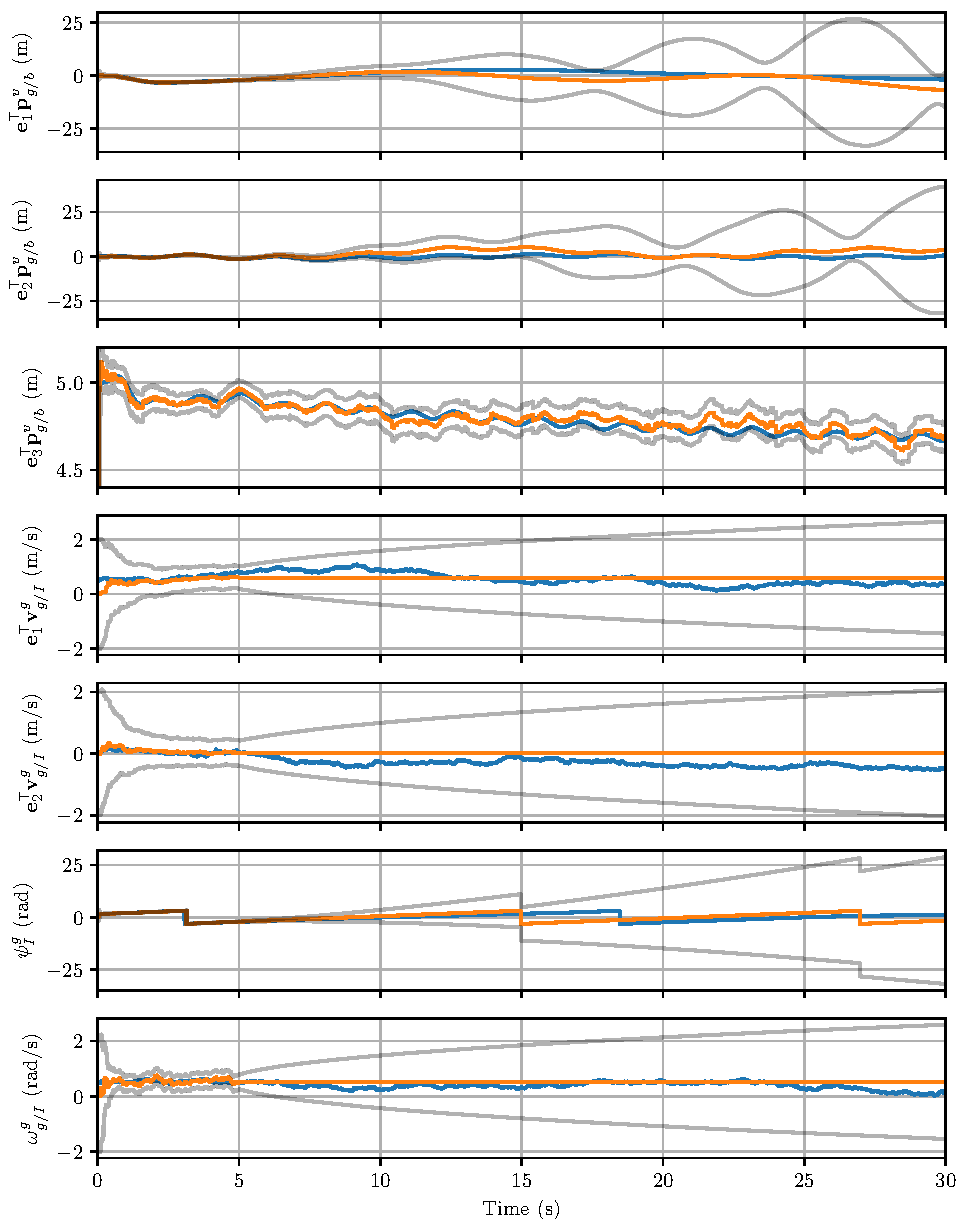
\includegraphics[width=6.5in]{plots/single_run_no_lms}
  \caption[ESKF Simulation Results Using No Visual Features]{Simulation results when the ESKF estimated the positions of \emph{no} visual
  features. The blue line represents the true state while the orange line
  represents the estimated state. The two grey lines show $\pm 2 \sigma$ bounds for
  the estimate based on the estimated covariance. Measurements from the fiducial
  marker were not used after $t = 5$ s
  to demonstrate the performance of the estimator.}
  \label{fig:no_lms}
\end{figure}

\begin{figure}
  \centering
  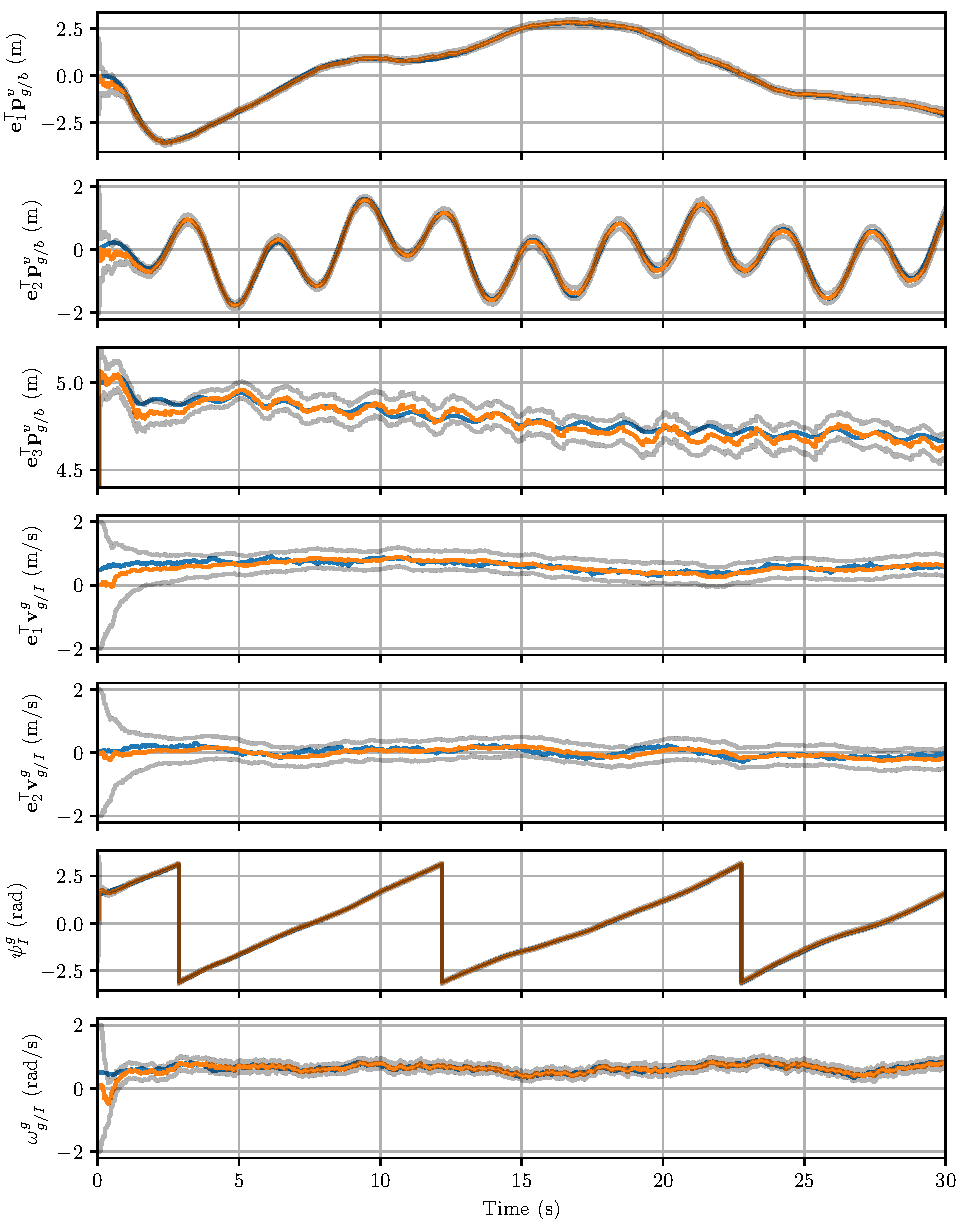
\includegraphics[width=6.5in]{plots/single_run_with_lms}
  \caption[ESKF Simulation Results Using Ten Visual Features]{Simulation results
    when the ESKF estimated the positions of \emph{ten} visual
  features. The blue line represents the true state while the orange line
  represents the estimated state. The two grey lines show $\pm 2 \sigma$ bounds for
  the estimate based on the estimated covariance. Measurements from the fiducial
  marker were not used after $t = 5$ s
  to demonstrate the performance of the estimator.}
  \label{fig:with_lms}
\end{figure}


% when the ESKF does not estimate
% the locations of any visual features ($n = 0$) in~\figref{fig:no_lms}, and 
% when the ESKF estimates the location of 10 visual features ($n =
% 10$) in~\figref{fig:with_lms}.
% Simulation experiments were performed with the ESKF
% The estimated state of the target vehicle, $\hat{\x}_{\text{Goal}}$, is seen in Figs.~\ref{fig:no_lms}
% and~\ref{fig:with_lms}, where~\figref{fig:no_lms} shows the results when the
% ESKF does not estimate any visual features ($n = 0$) and~\figref{fig:with_lms}
% shows the results when the ESKF estimates the locations of 10 visual features
% ($n = 10$).

% The simulation results for a 30 second simulation in which the estimator does
% not use any visual features are seen in
% Figures~\ref{fig:no_lms_gp}, \ref{fig:no_lms_gv}, \ref{fig:no_lms_gatt}. In the
% experiment shown, the measurements from the fiducial landing marker are not used
% after $t = 5 \hphantom{\cdot} s$ to demonstrate the performance of the proposed
% estimation algorithm when the fiducial marker is not detected for significant
% periods of time. The figures clearly show that when measurements from the
% fiducial marker are not available, the covariance of the estimate grows rapidly
% and the estimated state of the landing vehicle quickly becomes inaccurate. This
% matches our intuition as the estimator receives no information about the landing
% vehicle after $t = 5 \hphantom{\cdot} s$ and therefore is only able to propagate
% the dynamics of the system. We note that the $z$ direction of the estimated
% relative goal position is the exception as the landing vehicle is constrained to
% move only in the $xy$ plane. We do not include the plots of the estimated UAV states,
% $\hat{\x}_{\text{UAV}}$, as it is well known that these states are easily
% estimated with the given measurements.

% Simulation results for the same scenario, but in which the estimator uses a
% maximum of 10 visual features, are seen in
% Figures~\ref{fig:with_lms_gp}, \ref{fig:with_lms_gv}, \ref{fig:with_lms_gatt}.
% These figures clearly show that even after $t = 5 \hphantom{\cdot} s$ when the
% fiducial marker measurements are no longer available, the estimated states of
% the landing vehicle remain accurate with relatively tight covariance bounds. We
% reiterate that the only information the estimator receives during this time is
% the measured pixel locations of unknown visual features on the landing vehicle.

To further demonstrate performance, the two previous experiments were each
repeated 100 times.
The error in the estimated position of the target vehicle in the $xy$ plane of
the inertial frame is
plotted with respect to time for each of these experiments
in~\figref{fig:mc_xy_err}. While the error when $n = 10$
remained under one meter for all 100 simulations, the error when $n = 0$
grew quickly, reaching an error of over ten meters in many cases.
% runs of the same two
% experiments were performed.
% mentioned above were performed
% both using ten visual features and using zero visual features.
% The L2 norm of
% the $xy$ error of the estimated goal position state are plotted
% with respect to time in
% Figures~\ref{fig:mc_no_lms_xy_err}~and~\ref{fig:mc_with_lms_xy_err}. While the
% error when using 10 features
% almost entirely remains under 1 $m$ for all 100 simulations, the error when using
% no features quickly grows very large, reaching an error of over 10 $m$ in many
% of the runs.

\begin{figure}
  \centering
  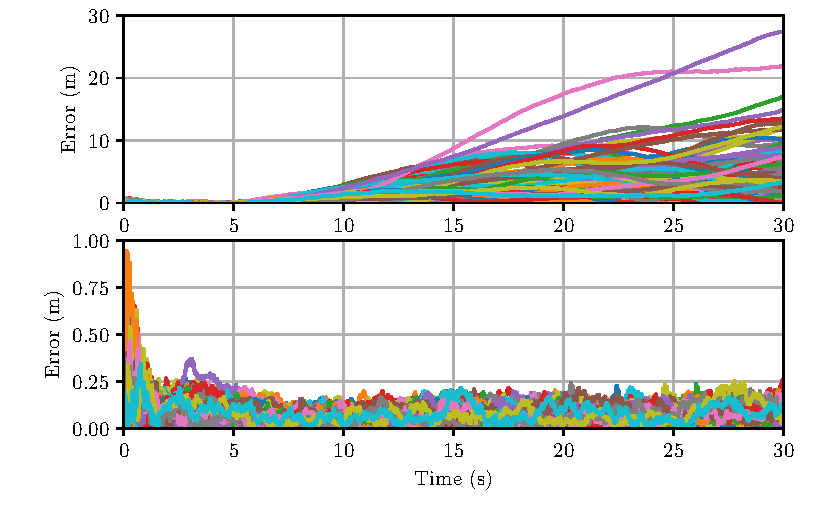
\includegraphics[width=5.5in]{plots/mc_both_xy_err}
  \caption[Estimated Error for 100 Simulations]{Error of the estimated position of the target vehicle in the $xy$
    plane. The top plot shows the error with respect to time for 100 simulations in which the ESKF
    estimates the positions of zero visual features. The bottom plot shows the
    error with respect to time for 100 simulations in which the ESKF estimates
    the positions of ten
    visual features.
    Measurements from the fiducial marker are not used after $t = 5$ s to
    demonstrate the performance of the estimator.
    % Simulation results with estimator using a maximum of ten visual
  % features. Measurements from the fiducial marker are not used after $t$ = 5
% $s$ to demonstrate the performance of the estimator. The L2 norm of the error in
% the x and y directions of the goal position is seen for 100 different simulation
% runs.
}
  \label{fig:mc_xy_err}
\end{figure}

